\documentclass[]{article}
\usepackage[brazil]{babel}
\usepackage[]{graphicx}
\usepackage{amsmath}

\title{Sistema de Alarme de Automóvel}
\author{Erickson Müller, mat: 20230001178\\ Nicole Moritz, mat: 2221101074}
\date{24 de abril de 2024}

\begin{document}
	\maketitle
	\pagebreak
	\section{Circuito}
		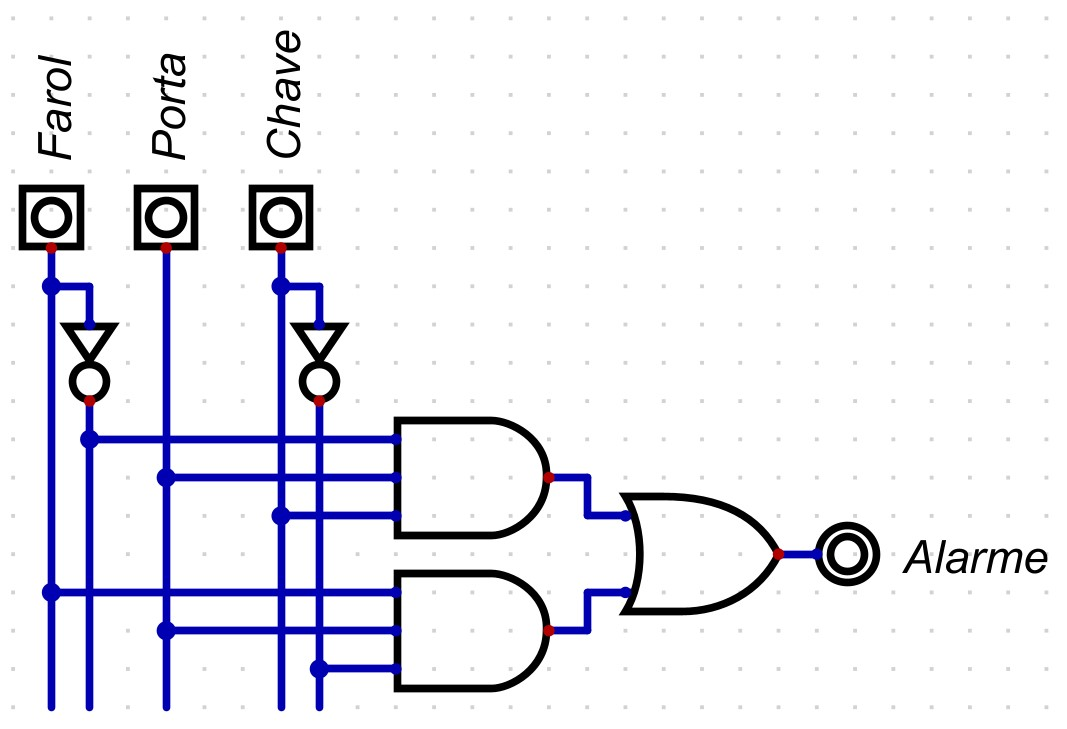
\includegraphics[scale=0.5]{Images/Circuito Alarme.jpg}
	\section{Tabela Verdade}
		\hspace*{4cm}
		\begin{tabular}{|c|c|c|c|}
			\hline
			\textbf{ F } & \textbf{ P } & \textbf{ C } & \textbf{ A } \\
			\hline
			0 & 0 & 0 & 0 \\
			\hline
			0 & 0 & 1 & 0 \\
			\hline
			0 & 1 & 0 & 0 \\
			\hline
			0 & 1 & 1 & 1 \\
			\hline
			1 & 0 & 0 & 0 \\
			\hline
			1 & 0 & 1 & 0 \\
			\hline
			1 & 1 & 0 & 1 \\
			\hline
			1 & 1 & 1 & 0 \\
			\hline
		\end{tabular}
	\\
	F = Farol \\ P = Porta \\ C = Chave \\ A = Alarme
	\pagebreak
	\section{Expressão}
		\begin{equation*}
			A = (\overline{F}.P.C) + (F.P.\overline{C})
		\end{equation*}
	\section{Circuitos Integrados}
	\section{Processo de Montagem em Plataforma Virtual}
		\subsection{Energização da Protoboard e Montagem das Entradas}
			1 = Farol \\ 2 = Porta \\ 3 = Chaves \\
			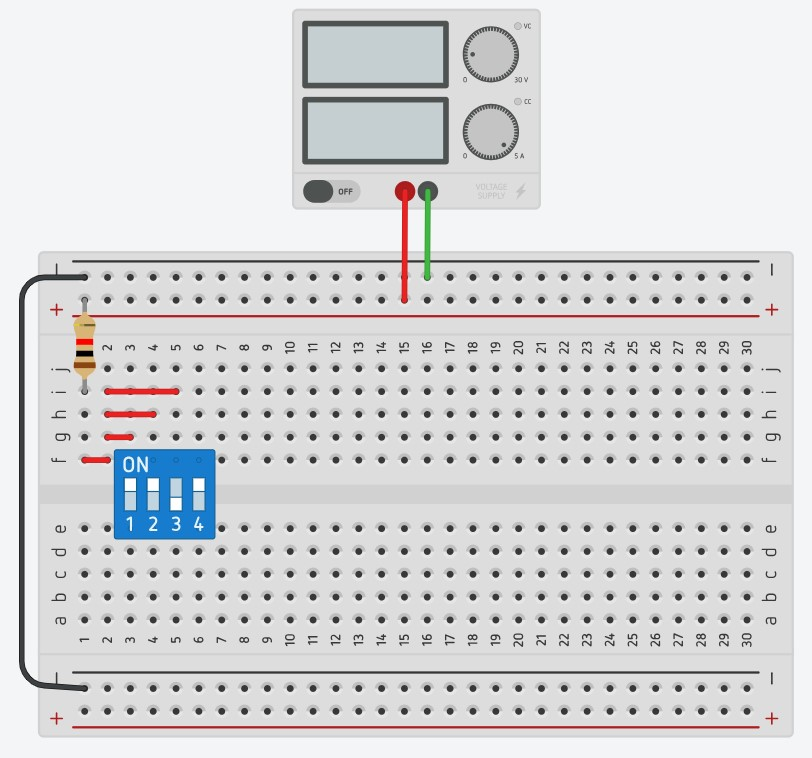
\includegraphics[scale=0.6]{Images/Tinkercad 01.jpg} \\
		\subsection{Porta Lógica NAND (CI 7400)}
			Essas portas lógicas são necessárias para inverter os valores das entradas 1 (Farol, representado pelo fio amarelo) e 3 (Chave na ignição, representado pelo fio verde) \\
			A CI foi energizada puxando da linha 2 da parte superior e aterrando no negativo da parte inferior. \\
			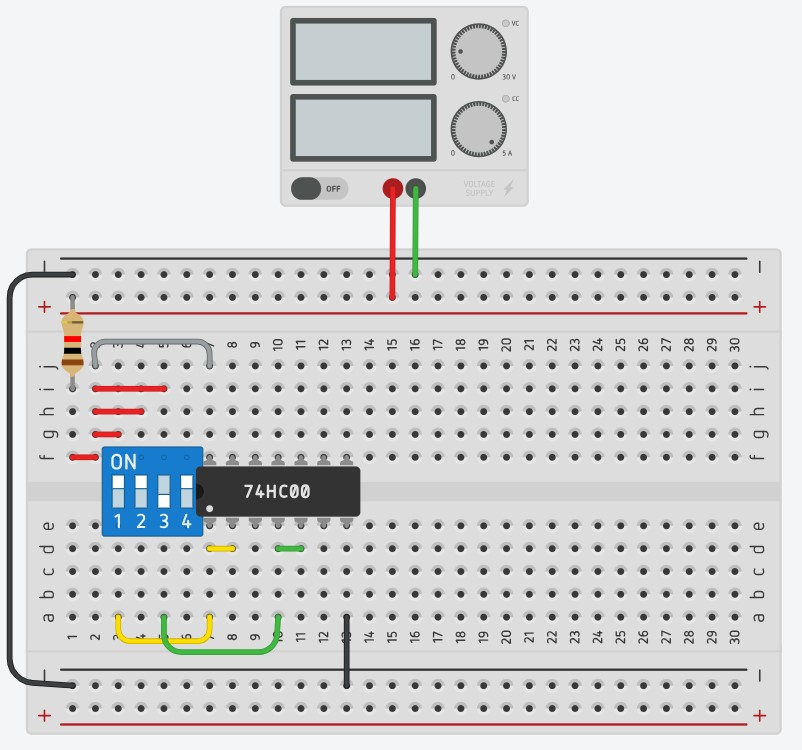
\includegraphics[scale=0.6]{Images/Tinkercad 02.jpg} \\
		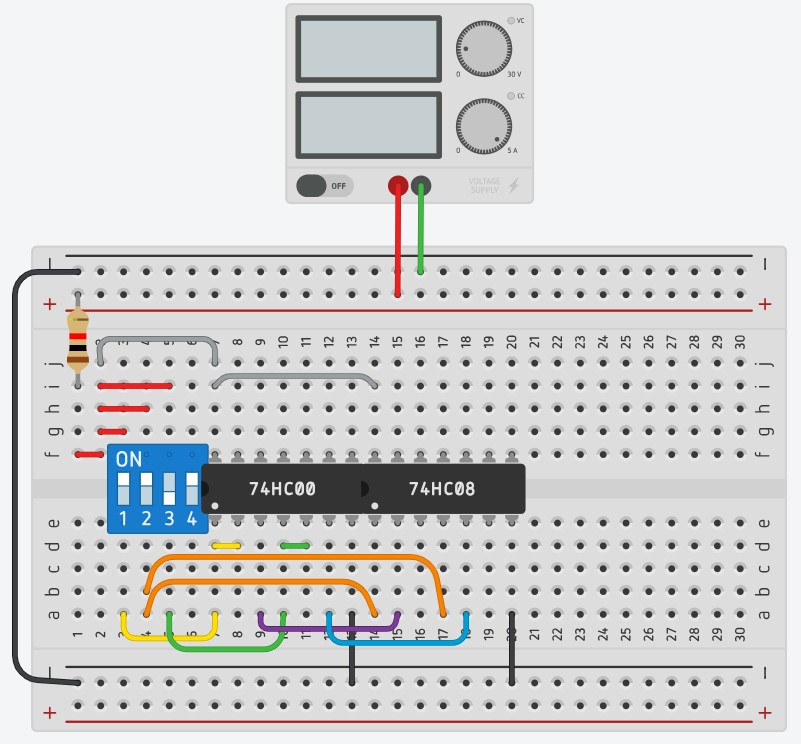
\includegraphics[scale=0.6]{Images/Tinkercad 03.jpg} \\
		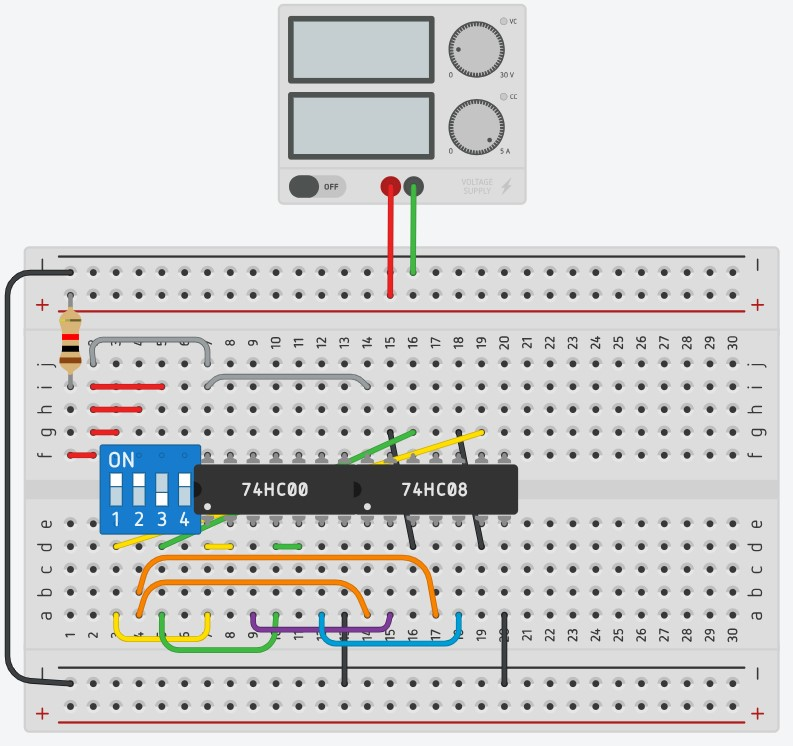
\includegraphics[scale=0.6]{Images/Tinkercad 04.jpg} \\
		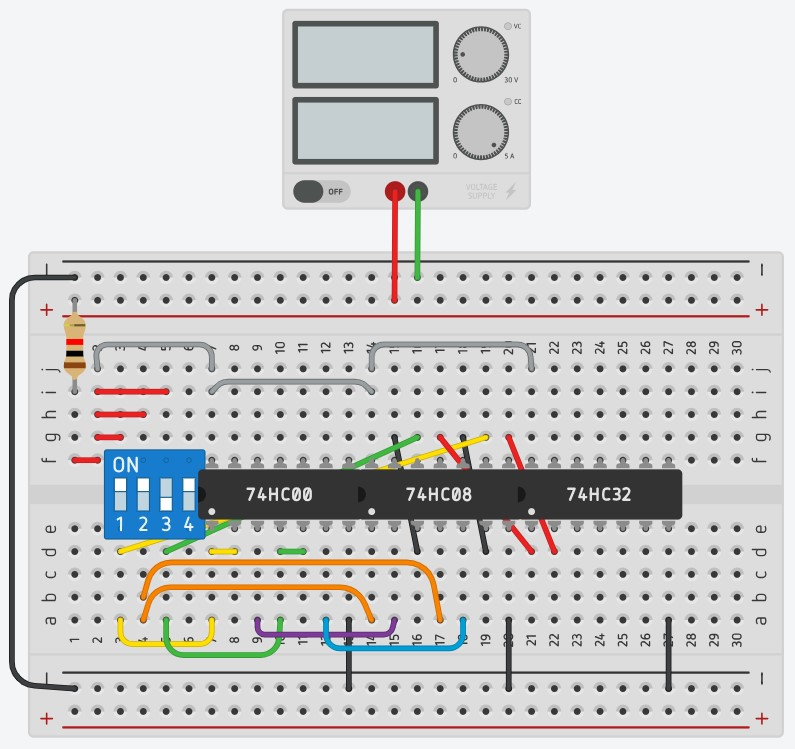
\includegraphics[scale=0.6]{Images/Tinkercad 05.jpg} \\
		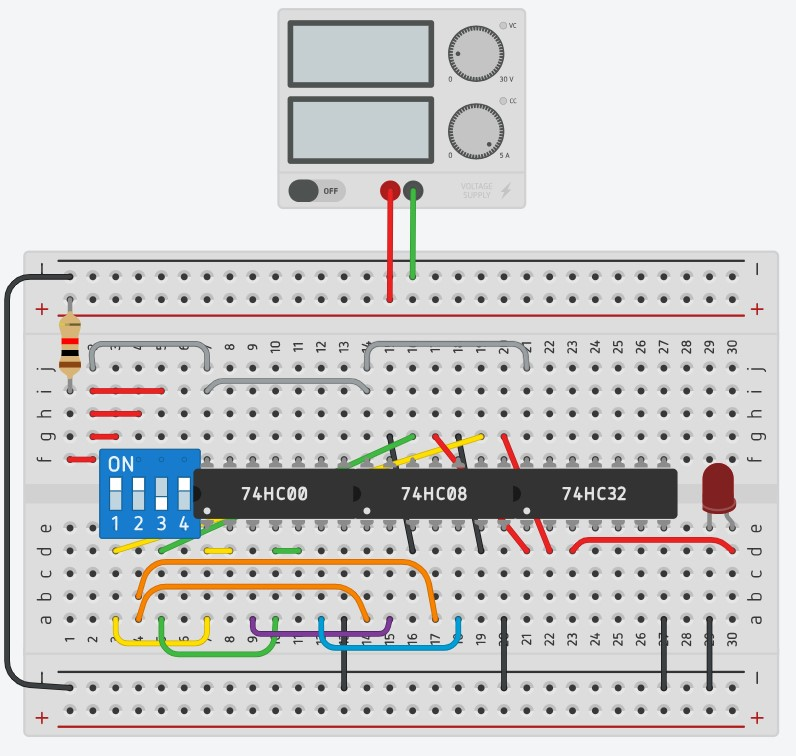
\includegraphics[scale=0.6]{Images/Tinkercad 06.jpg} \\
	\section{Circuito na Protoboard}
	
\end{document}